\section{Experiments}
\label{sec:experiments}
We evaluate our SupCon loss ($\mathcal{L}_{out}^{sup}$, Eq. \ref{eqn:supervised_loss}) by measuring classification accuracy on a number of common image classification benchmarks including CIFAR-10 and CIFAR-100 \cite{krizhevsky2009learning} and ImageNet \cite{deng2009imagenet}. We also benchmark our ImageNet models on robustness to common image corruptions \cite{hendrycks2019benchmarking} and show how performance varies with changes to hyperparameters and reduced data. For the encoder network ($Enc(\cdot)$) we experimented with three commonly used encoder architectures: ResNet-50, ResNet-101, and ResNet-200 \cite{he2016deep}. The normalized activations of the final pooling layer ($D_E=2048$) are used as the representation vector. We experimented with four different implementations of the $Aug(\cdot)$ data augmentation module: AutoAugment \cite{cubuk2019autoaugment}; RandAugment \cite{cubuk2019randaugment}; SimAugment \cite{chen2020simple}, and Stacked RandAugment \cite{tian2020makes} (see details of our SimAugment and Stacked RandAugment implementations in the Supplementary). AutoAugment outperforms all other data augmentation strategies on ResNet-50 for both SupCon and cross-entropy. Stacked RandAugment performed best for ResNet-200 for both loss functions. We provide more details in the Supplementary.



\subsection{Classification Accuracy}
Table \ref{tab:datasets} shows that SupCon generalizes better than cross-entropy, margin classifiers (with use of labels) and unsupervised contrastive learning techniques on CIFAR-10, CIFAR-100 and ImageNet datasets. Table \ref{table:imagenet_top1} shows results for ResNet-50 and ResNet-200 (we use ResNet-v1 \cite{he2016deep}) for ImageNet. We achieve a new state of the art accuracy of $78.7\%$ on ResNet-50 with AutoAugment (for comparison, a number of the other top-performing methods are shown in Fig. \ref{fig:imagenet_top1_teaser}). Note that we also achieve a slight improvement over CutMix \cite{yun2019cutmix}, which is considered to be a state of the art data augmentation strategy. Incorporating data augmentation strategies such as CutMix \cite{yun2019cutmix} and MixUp \cite{zhang2017mixup} into contrastive learning could potentially improve results further. 

We also experimented with memory based alternatives \cite{he2019momentum}. On ImageNet, with a memory size of 8192 (requiring only the storage of 128-dimensional vectors), a batch size of 256, and SGD optimizer, running on 8 Nvidia V100 GPUs, SupCon is able to achieve $79.1\%$ top-1 accuracy on ResNet-50. This is in fact slightly better than the $78.7\%$ accuracy with 6144 batch size (and no memory);
and with significantly reduced compute and memory footprint.

Since SupCon uses 2 views per sample, its batch sizes are effectively twice the cross-entropy equivalent. We therefore also experimented with the cross-entropy ResNet-50 baselines using a batch size of 12,288. These only achieved $77.5\%$ top-1 accuracy. We additionally experimented with increasing the number of training epochs for cross-entropy all the way to 1400, but this actually decreased accuracy ($77.0\%$).

We tested the N-pairs loss \cite{sohn2016improved} in our framework with a batch size of 6144. N-pairs achieves only $57.4\%$ top-1 accuracy on ImageNet. We believe this is due to multiple factors missing from N-pairs loss compared to supervised contrastive: the use of multiple views; lower temperature; and many more positives. We show some results of the impact of the number of positives per anchor in the Supplementary (Sec. 6), and the N-pairs result is inline with them. We also note that the original N-pairs paper \cite{sohn2016improved} has already shown the outperformance of N-pairs loss to triplet loss. 

\begin{table}[t]
    \centering
     \vspace{-5pt}
    \begin{tabular}{ccccc}
        \toprule
        Dataset & SimCLR\cite{chen2020simple} & Cross-Entropy & Max-Margin \cite{liu2016largemargin}  &  SupCon \\\midrule
        CIFAR10  & 93.6 & 95.0 & 92.4 & \bf{96.0} \\
        CIFAR100 & 70.7 & 75.3 & 70.5 & \bf{76.5} \\
        ImageNet & 70.2 & 78.2 & 78.0 & \bf{78.7} \\
        \bottomrule
    \end{tabular}
    \vspace{2mm}
    \caption{Top-1 classification accuracy on ResNet-50 \cite{he2016deep} for various datasets. We compare cross-entropy training, unsupervised representation learning (SimCLR \cite{chen2020simple}), max-margin classifiers \cite{liu2016largemargin} and SupCon (ours). We re-implemented and tuned hyperparameters for all baseline numbers except margin classifiers where we report published results.  Note that the CIFAR-10 and CIFAR-100 results are from our PyTorch implementation and ImageNet from our TensorFlow implementation.}
    \vspace{-5pt}
    \label{tab:datasets}
\end{table}


\begin{table}[t]
 \vspace{-10pt}
\centering
\begin{tabular}{ccccc} 
 \toprule
  Loss & Architecture & Augmentation & Top-1 & Top-5 \\\midrule
 Cross-Entropy (baseline) & ResNet-50  & MixUp \cite{zhang2017mixup} & 77.4 & 93.6 \\
 Cross-Entropy (baseline) & ResNet-50 & CutMix \cite{yun2019cutmix} & 78.6 & 94.1 \\
 Cross-Entropy  (baseline) & ResNet-50 & AutoAugment \cite{cubuk2019autoaugment} & 78.2 & 92.9 \\
 Cross-Entropy (our impl.) & ResNet-50 & AutoAugment \cite{lim2019fast} & 77.6 & 95.3 \\ 
 SupCon & ResNet-50 & AutoAugment \cite{cubuk2019autoaugment}
 & {\bf 78.7} & {\bf 94.3} \\ \midrule
 Cross-Entropy (baseline) & ResNet-200 & AutoAugment \cite{cubuk2019autoaugment} & 80.6 & 95.3 \\ 
 Cross-Entropy (our impl.) & ResNet-200 & Stacked RandAugment \cite{tian2020makes} & 80.9 & 95.2 \\ 
 SupCon & ResNet-200 & Stacked RandAugment \cite{tian2020makes}
 & {\bf 81.4} & {\bf 95.9} \\ \midrule
 SupCon & ResNet-101 & Stacked RandAugment \cite{tian2020makes} & 80.2 & 94.7 \\ \bottomrule
 
\end{tabular}
\vspace{2mm}
\caption{Top-1/Top-5 accuracy results on ImageNet for AutoAugment \cite{cubuk2019autoaugment} with ResNet-50 and for Stacked RandAugment \cite{tian2020makes} with ResNet-101 and ResNet-200. The baseline numbers are taken from the referenced papers, and we also re-implement cross-entropy.}
 \vspace{-20pt}
\label{table:imagenet_top1}
\end{table}

 

\begin{figure}[t]
\centering
\begin{minipage}[t]{.6\linewidth}
\small
\setlength{\tabcolsep}{2pt}
\vspace{0pt}
\centering
\begin{tabular}{cccc} 
 \toprule
  Loss & Architecture & rel. mCE & mCE \\\midrule
 Cross-Entropy & AlexNet \cite{krizhevsky2012imagenet} & 100.0 & 100.0 \\
 (baselines)& VGG-19+BN \cite{Simonyan15} & 122.9 & 81.6 \\
 & ResNet-18 \cite{he2016deep} & 103.9 & 84.7 \\\midrule
 Cross-Entropy & ResNet-50 & 96.2 & 68.6 \\
 (our implementation)& ResNet-200 & 69.1 & 52.4 \\ 
 \midrule
 Supervised Contrastive & ResNet-50 & {\bf 94.6} & {\bf 67.2} \\
 & ResNet-200 & {\bf 66.5} & {\bf 50.6} \\ \bottomrule
\end{tabular}
\end{minipage}%
\begin{minipage}[t]{.4\linewidth}
\vspace{0pt}
\centering
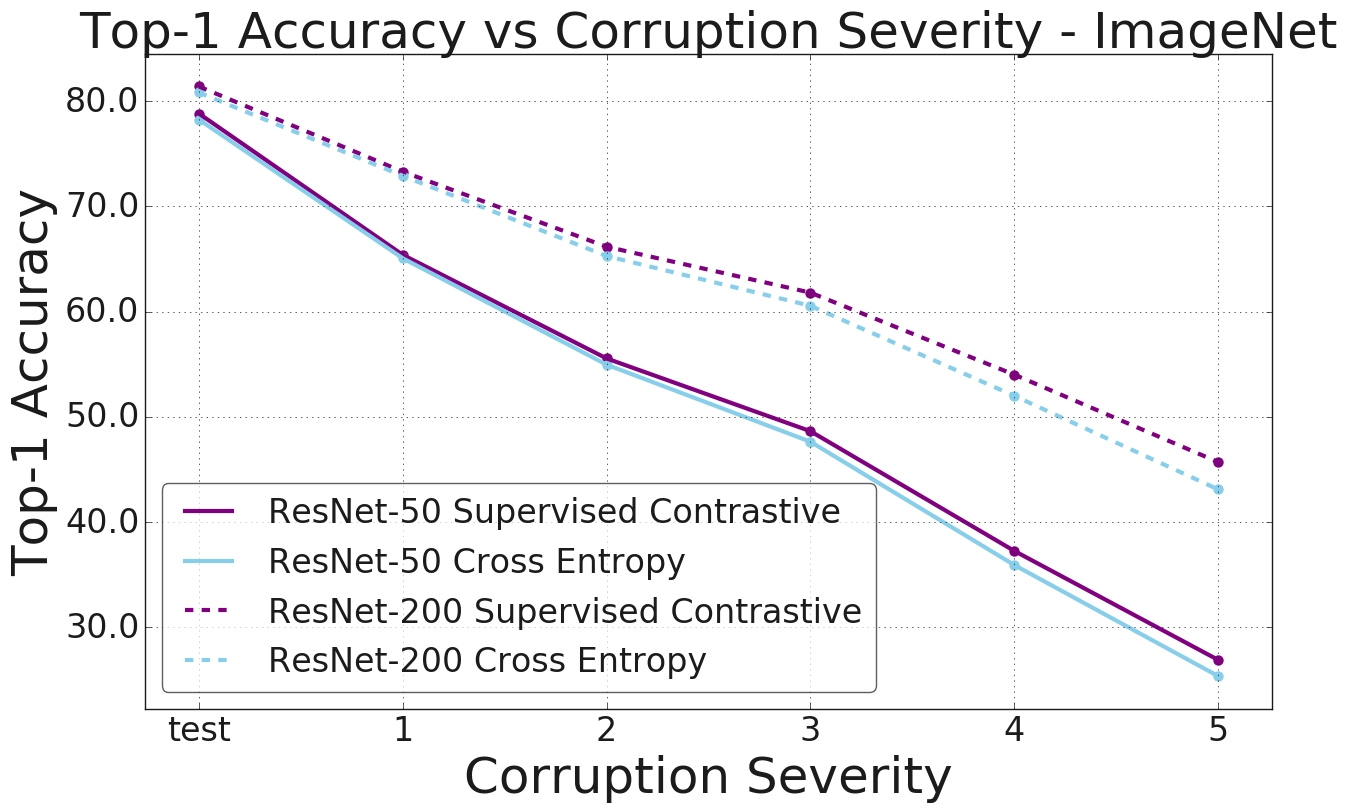
\includegraphics[width=0.9\linewidth]{figs/corrupt_top1.png}
\end{minipage}

\caption{ Training with supervised contrastive loss makes models more robust to corruptions in images. {\bf Left}: Robustness as measured by Mean Corruption Error (mCE) and relative mCE over the ImageNet-C dataset \cite{hendrycks2019benchmarking} (lower is better). {\bf Right}: Mean Accuracy as a function of corruption severity averaged over all various corruptions. (higher is better).}
\label{table:robustness}

\end{figure}

\subsection{Robustness to Image Corruptions and Reduced Training Data}
Deep neural networks lack robustness to out of distribution data or natural corruptions such as noise, blur and JPEG compression. The benchmark ImageNet-C dataset \cite{hendrycks2019benchmarking} is used to measure trained model performance on such corruptions. In Fig. \ref{table:robustness}(left), we compare the supervised contrastive models to cross-entropy using the Mean Corruption Error (mCE) and Relative Mean Corruption Error metrics \cite{hendrycks2019benchmarking}. Both metrics measure average degradation in performance compared to ImageNet test set, averaged over all possible corruptions and severity levels. Relative mCE is a better metric when we compare models with different Top-1 accuracy, while mCE is a better measure of absolute robustness to corruptions. The SupCon models have lower mCE values across different corruptions, showing increased robustness. We also see from Fig. \ref{table:robustness}(right) that SupCon models demonstrate lesser degradation in accuracy with increasing corruption severity. 


\begin{figure}
    \centering
    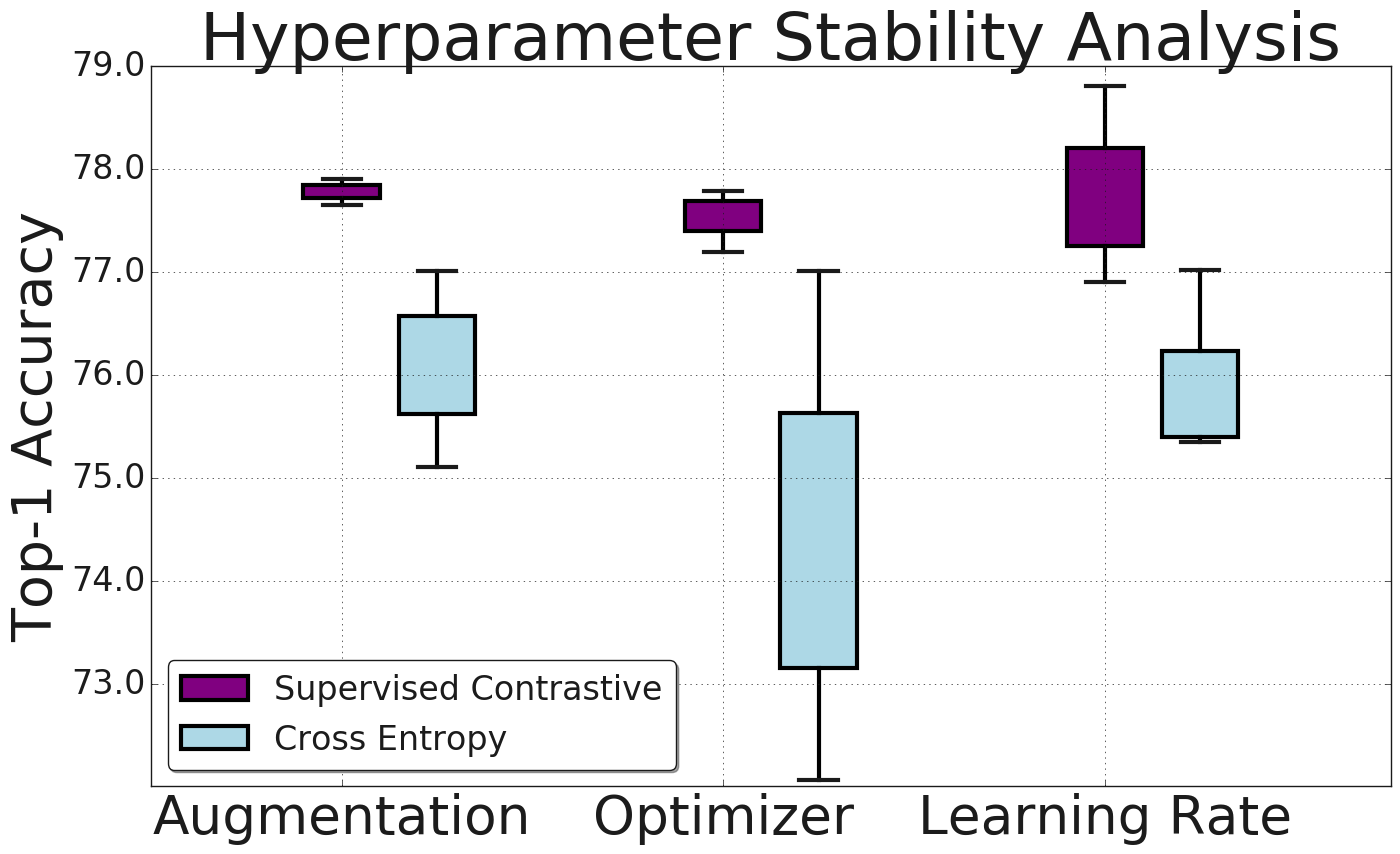
\includegraphics[width=0.24\linewidth]{figs/stability.png}
    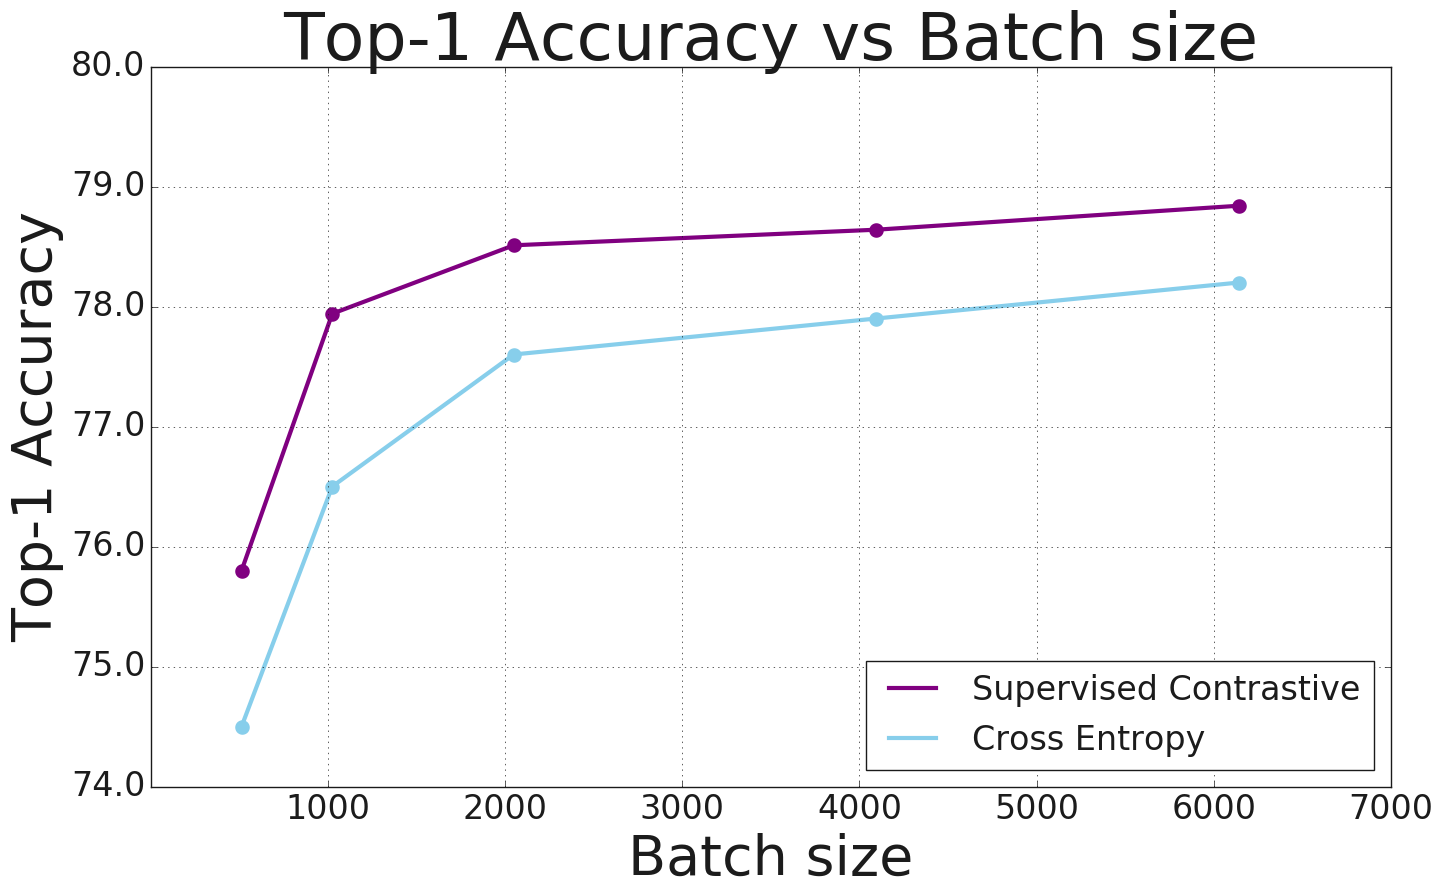
\includegraphics[width=0.24\linewidth]{figs/top1-vs-bs.png}
    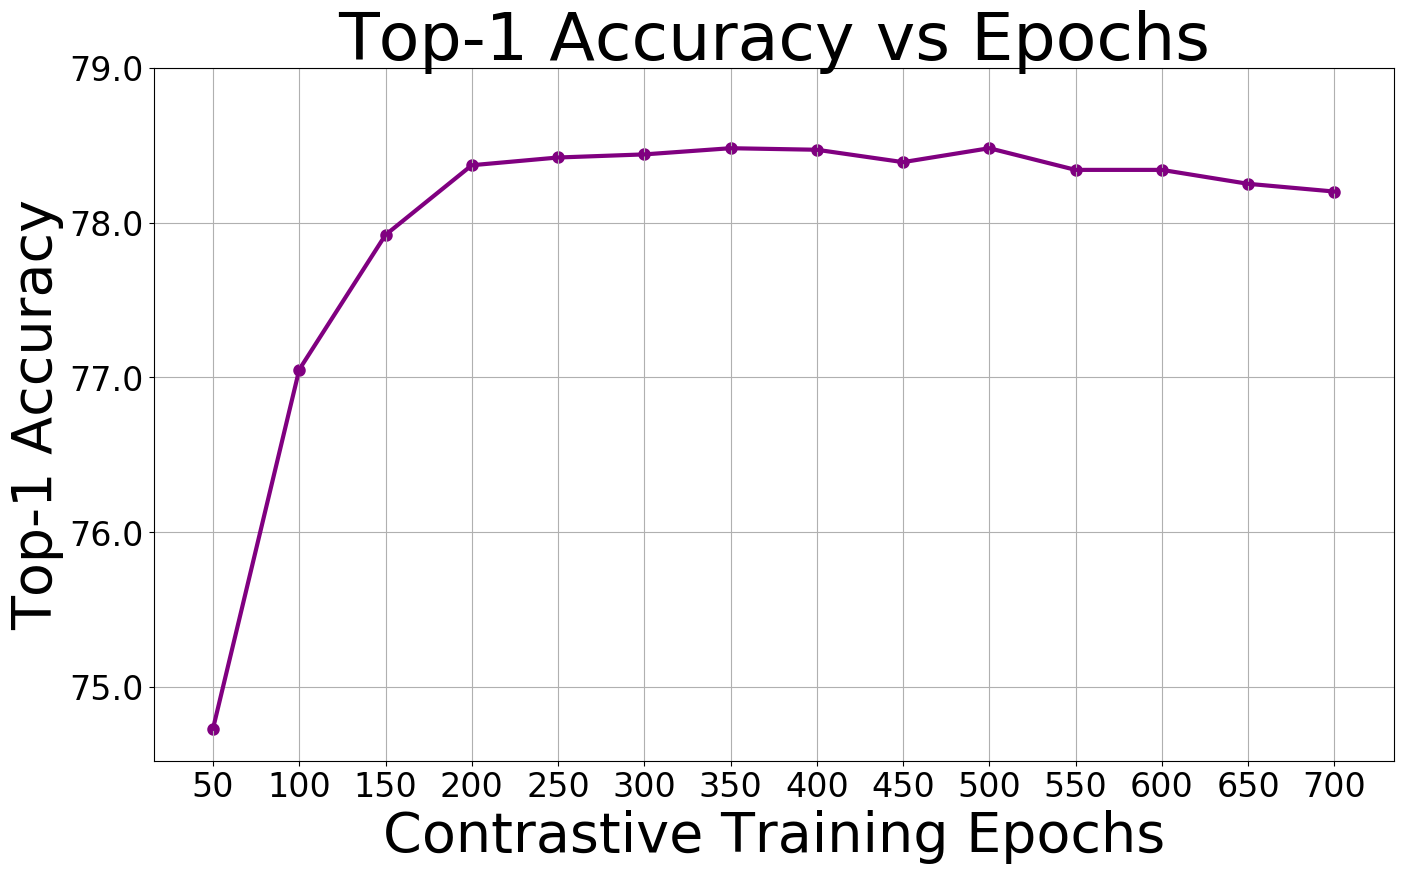
\includegraphics[width=0.24\linewidth]{figs/epoch_sweep.png}
    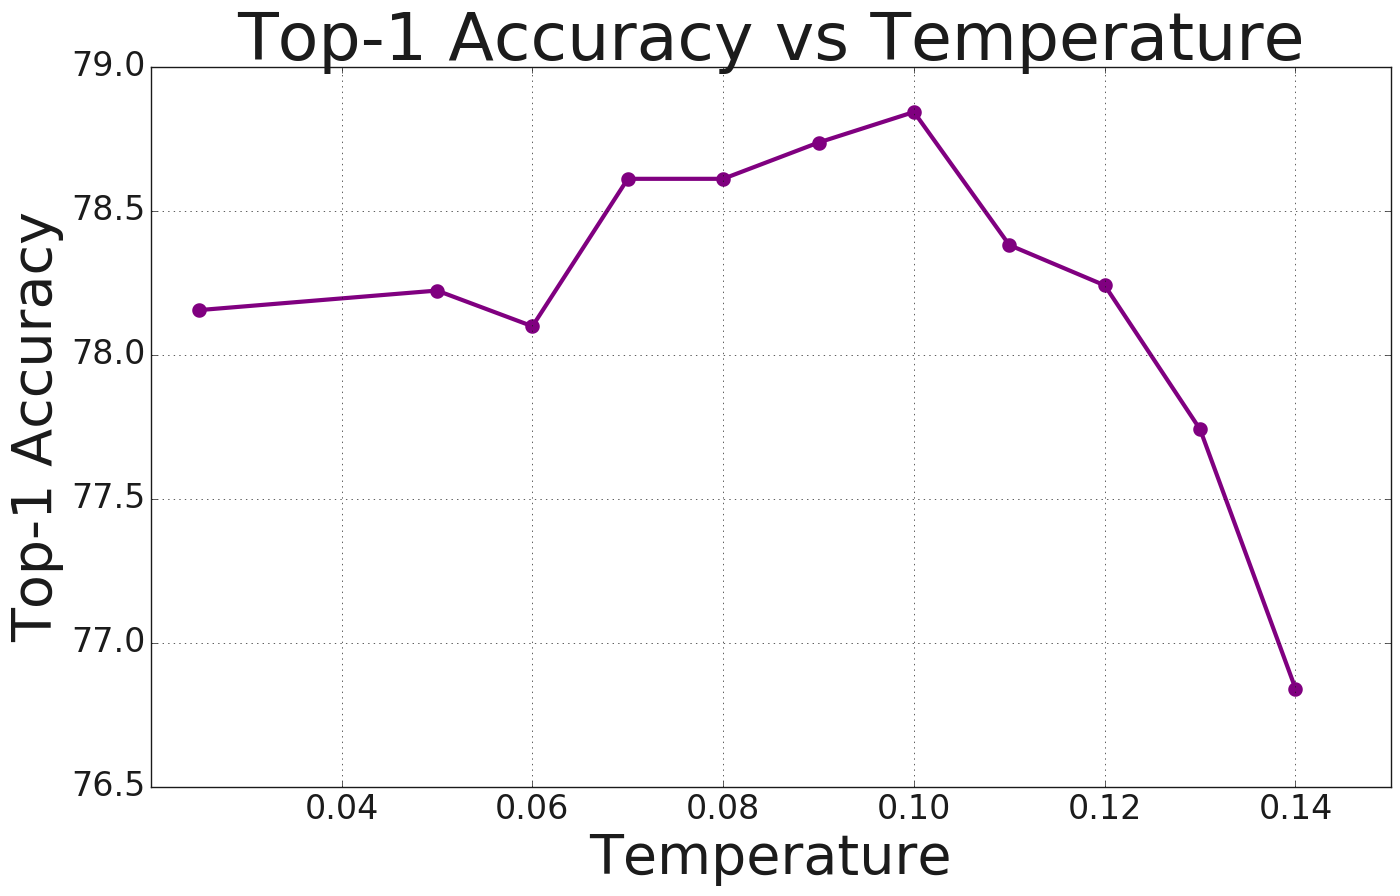
\includegraphics[width=0.24\linewidth]{figs/temperature.png}
    \caption{Accuracy of cross-entropy and supervised contrastive loss as a function of hyperparameters and training data size, all measured on ImageNet with a ResNet-50 encoder. (From left to right)
    {\bf (a)}: Standard boxplot showing Top-1 accuracy vs changes in augmentation, optimizer and learning rates. 
    {\bf (b)}: Top-1 accuracy as a function of batch size shows both losses benefit from larger batch sizes while Supervised Contrastive has higher Top-1 accuracy even when trained with smaller batch sizes. 
    {\bf (c)}: Top-1 accuracy as a function of SupCon pretraining epochs.
     {\bf (d)}: Top-1 accuracy as a function of temperature during pretraining stage for SupCon. 
     }
    % \vspace{-10pt}
    \label{fig:hparam_stability} 
\end{figure}





\subsection{Hyperparameter Stability}
We experimented with hyperparameter stability by changing augmentations, optimizers and learning rates one at a time from the best combination for each of the methodologies. In Fig. \ref{fig:hparam_stability}(a), we compare the top-1 accuracy of SupCon loss against cross-entropy across changes in augmentations (RandAugment \cite{cubuk2019randaugment}, AutoAugment \cite{cubuk2019autoaugment}, SimAugment \cite{chen2020simple}, Stacked RandAugment \cite{tian2020makes}); optimizers (LARS, SGD with Momentum and RMSProp); and learning rates. We observe significantly lower variance in the output of the contrastive loss. Note that batch sizes for cross-entropy and supervised contrastive are the same, thus ruling out any batch-size effects. In Fig. \ref{fig:hparam_stability}(b), sweeping batch size and holding all other hyperparameters constant results in consistently better top-1 accuracy of the supervised contrastive loss.


\subsection{Transfer Learning}
We evaluate the learned representation for fine-tuning on 12 natural image datasets, following the protocol in Chen et.al. \cite{chen2020simple}. SupCon is on par with cross-entropy and \emph{self-supervised} contrastive loss on transfer learning performance when trained on the same architecture (Table \ref{table:transfer}). Our results are consistent with the findings in \cite{he2019rethinking} and \cite{kornblith2019better}: while better ImageNet models are correlated with better transfer performance, the dominant factor is architecture. Understanding the connection between training objective and transfer performance is left to future work. 

\begin{table}[t!]
\scriptsize
\setlength{\tabcolsep}{2pt}
\begin{tabular}{cccccccccccccc} 
 \toprule
   & Food & CIFAR10 & CIFAR100  & Birdsnap & SUN397 & Cars & Aircraft & VOC2007 & DTD & Pets & Caltech-101 & Flowers & Mean \\\midrule
 SimCLR-50 \cite{chen2020simple} &  \textbf{88.20} & \textbf{97.70} & \textbf{85.90} & \textbf{75.90} & \textbf{63.50} & 91.30 & \textbf{88.10} & 84.10 & 73.20 & 89.20 & 92.10 & \textbf{97.00} & \textbf{84.81}\\ 
 Xent-50 & 87.38 &	96.50 &	84.93 &	74.70 &	63.15 &	89.57 &	80.80 &	\textbf{85.36} &	\textbf{76.86} &	92.35 &	\textbf{92.34} &	96.93 & \textbf{84.67}\\
  SupCon-50 & 87.23 &	97.42 &	84.27 &	75.15 &	58.04 &	\textbf{91.69} &	84.09 &	85.17 &	74.60 &	\textbf{93.47} &	91.04 &	96.0 & \textbf{84.27}\\
 \midrule
 Xent-200 &  \textbf{89.36} &	97.96 &	86.49 &	\textbf{76.50} &	\textbf{64.36}  & 90.01 & 84.22 & \textbf{86.27} & \textbf{76.76} & \textbf{93.48} & 93.84 & \textbf{97.20} &  \textbf{85.77}\\
  SupCon-200 &  88.62 & \textbf{98.28} & \textbf{87.28} & 76.26 & 60.46 & \textbf{91.78} & \textbf{88.68} & 85.18 & 74.26 & 93.12 & \textbf{94.91} & 96.97 & \textbf{85.67}\\
  \bottomrule
\end{tabular}


\vspace{2mm}
\caption{Transfer learning results.  Numbers are mAP for VOC2007 \cite{pascal-voc-2007}; mean-per-class accuracy for Aircraft, Pets, Caltech, and Flowers; and top-1 accuracy for all other datasets.} %
\vspace{-22pt}
\label{table:transfer}
\end{table}


\subsection{Training Details}
The SupCon loss was trained for $700$ epochs during pretraining for ResNet-200 and $350$ epochs for smaller models. Fig. \ref{fig:hparam_stability}(c) shows accuracy as a function of SupCon training epochs for a ResNet50, demonstrating that even 200 epochs is likely sufficient for most purposes.

An (optional) additional step of training a linear classifier is used to compute top-1 accuracy. This is not needed if the purpose is to use representations for transfer learning tasks or retrieval. The second stage needs as few as 10 epochs of additional training. Note that in practice the linear classifier can be trained jointly with the encoder and projection networks by blocking gradient propagation from the linear classifier back to the encoder, and achieve roughly the same results without requiring two-stage training. We chose not to do that here to help isolate the effects of the SupCon loss.

We trained our models with batch sizes of up to 6144, although batch sizes of 2048 suffice for most purposes for both SupCon and cross-entropy losses (as shown in Fig. \ref{fig:hparam_stability}(b)). We associate some of the performance increase with batch size to the effect on the gradient due to hard positives increasing with an increasing number of negatives (see the Supplementary for details). We report metrics for experiments with batch size $6144$ for ResNet-50 and batch size $4096$ for ResNet-200 (due to the larger network size, a smaller batch size is necessary). We observed that for a fixed batch size it was possible to train with SupCon using larger learning rates than what was required by cross-entropy to achieve similar performance.

All our results used a temperature of $\tau = 0.1$. Smaller temperature benefits training more than higher ones, but extremely low temperatures are harder to train due to numerical instability. Fig. \ref{fig:hparam_stability}(d) shows the effect of temperature on Top-1 performance of supervised contrastive learning. As we can see from Eq. \ref{eqn:gradient}, the gradient scales inversely with choice of temperature $\tau$; therefore we rescale the loss by $\tau$ during training for stability.

We experimented with standard optimizers such as LARS \cite{you2017large}, RMSProp \cite{hinton2012neural} and SGD with momentum \cite{ruder2016overview} in different permutations for the initial pre-training step and training of the dense layer. While SGD with momentum works best for training ResNets with cross-entropy, we get the best performance for SupCon on ImageNet by using LARS for pre-training and RMSProp to training the linear layer. For CIFAR10 and CIFAR100 SGD with momentum performed best. Additional results for combinations of optimizers are provided in the Supplementary. Reference code is released at \url{https://t.ly/supcon}. 